\section{Natural Language Processing (NLP)}
\subsection{Ingredients of Machine Learning}
\textbf{1. Data}
\begin{itemize}
    \item Dataset
    \item Pre-Processing Pipe-Line including cleansing, feature-engineering, data augmentation etc.
\end{itemize}
\textbf{2. Cost-Function (Loss)}
\begin{itemize}
    \item Formal mathematical expression for good / bad
    \item Commonly Mean Squared Error (MSE)
\end{itemize}
\textbf{3. Model}
\begin{itemize}
    \item From linear model: $\hat{y_i} = ax_i + b$
    \item To complicated million parameter neural networks
    \item Different tasks require different models (regression / decision tree)
\end{itemize}
\textbf{4. Optimization Procedure}
\begin{itemize}
    \item Algorithm that changes the parameters of the model that the cost-function is minimized.
    \item E.g. Stochastic Gradient Descent (SGD), ADAM, RMSProp...
\end{itemize}

\subsection{More ingredients}
For successful ML, there are many more ingredients:\\ 
\textbf{5. Performance optimization}
\begin{itemize}
    \item Building of efficient pipe-lines
    \item Folowwing tool specific recommendations
\end{itemize}
\textbf{6. Visualization and evaluation of the learning Process}
\begin{itemize}
    \item Learning curves
    \item Performance measures
    \item Tensorboard
\end{itemize}
\textbf{7. Cross-Validation \& Regularization}
\begin{itemize}
    \item Train models that generalize well to unseen data
    \item Estimate the generalization error
\end{itemize}

\subsection{Representation of Words}
Vectors can be used to represent words based on their meaning.
\subsubsection{One-hot representation}
\begin{itemize}
    \item Vector with a single 1-Value
    \item All other Values are set to 0
    \item Count the Number of different Words, Define one unique vector per word:
\end{itemize}
\textit{Dini Mom isch fett.}\\
Dini: $\begin{bmatrix} 1\\ 0\\ 0\\ 0\\ 0\end{bmatrix}$
Mom: $\begin{bmatrix} 0\\ 1\\ 0\\ 0\\ 0\end{bmatrix}$
isch: $\begin{bmatrix} 0\\ 0\\ 1\\ 0\\ 0\end{bmatrix}$
fett: $\begin{bmatrix} 0\\ 0\\ 0\\ 1\\ 0\end{bmatrix}$
'.': $\begin{bmatrix} 0\\ 0\\ 0\\ 0\\ 1\end{bmatrix}$\\ 
\textbf{Disadvantages:}
\begin{itemize}
    \item Very high dimensional vector space (1 Dimension / unique Word)
    \item Sparse Representation: Eech vector has a single 1 and $N$ Zeroes. (Memory Inefficient)
    \item No Generalization: All words are unrelated to each other.
    \item Does not capture any aspect of the meaning of a word
\end{itemize}

\subsubsection{Indexing}
Make a list of words (optionally alphabetically). Use the index to represent each word.\\ 
\textbf{Example:}\\
\textit{Dini Mom isch fett.}\\ 
Dini: $0$, Mom: $1$, isch: $2$, fett: $3$, '.': $4$
\begin{itemize}
    \item Dense Equivalent of one-hot encoding
    \item Indexes are not more useful that one-hot vectors
    \item Often used as preprocessing step
    \item Indices / One-Hot Vectors are fed into a network which learns more useful representations
\end{itemize}

\subsubsection{Distributed Representation}
\begin{itemize}
    \item Words that occur in similar contexts (neighboring words) tend to have similar meanings
    \item Similar words share similar representations
    \item Distributed representations can be learned
\end{itemize}
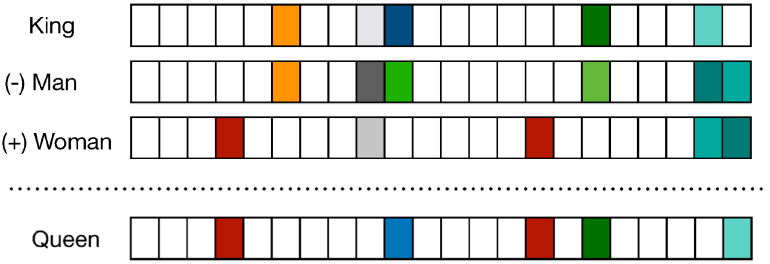
\includegraphics[width=.8\linewidth]{./img/distributed_representation.png}\\
\textbf{Words to Vectors:}
\begin{itemize}
    \item Mathematical function maps word to high dimensional Vector
    \item In neural networks, this function is implemented in the Embedding Layer
\end{itemize}
\textbf{Advantage of Vectors}
\begin{itemize}
    \item Good embedding maps simiar/related words to similar regions of the vector space
    \item Dot-Product (Skalarprodukt) is a measure of similarity
    \item Possible to add/subtract vectors
\end{itemize}
\textbf{Calculate Similarities between words}
Dot-Product (Skalarprodukt) of 2 Vectors:
\begin{itemize}
    \item maximal when parallel (0\textdegree) (1 with norm (length) 1)
    \item zero when orthogonal (90\textdegree)
    \item minimal (negative) when opposite directions (180\textdegree) (-1 with norm (length) 1)
\end{itemize}
\textbf{Cosine Distance}
\begin{itemize}
    \item Way to calculate how similar two words (vectors) are
\end{itemize}
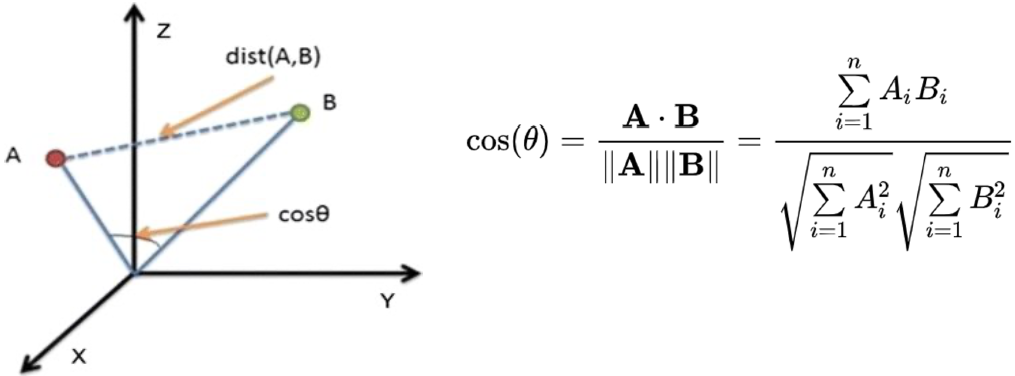
\includegraphics[width=\linewidth]{./img/cosine_distance.png}